\section{Insights from the features}
From the above explored visual, higher level features, it seems that there are a few aesthetic and affective properties of a video, that seem to be over expressed in a popular vine. The idea of vine is a micro video website, but the interpretation and projection of these microvideos as an art from is kept completely open to the users. It is in such sandboxes, interesting art is created. YouTube began with a similar motive and it has now evolved into a gargantuan platform for showcasing different artforms that trancent national bountries, languanges generes. Vine takes this one step further and ristricts the time. This can be a limiting factor or can be used in a peculiar way. Clearly it is the former as some of these videos get likes, shares and loops on par with famous viral videos. The question is what are these unique styles of the users that have allowed them to breach this ristriction. 
\par 
From the initial work done on aesthetic and affective aspects of a vine video in our paper, it seems the popularity is less of a function of aesthetics, but more of the content. Apart from colour contrast, none of the 9 major aesthetic parameters evaluated for both popular and unpopular vines, showed any form of over expression \ref{aesthetic_table}. Most parameters either were at par aestheic baseline images or fell way behind. But between the unpopular and popular set, there was hardly any formidable statistical difference. 
\par 
One major property that shows its presence was the presence of a human face \ref{fig:Face_CDF}. Popular videos show a very high bias towards videos with human faces in them. This says a something about why the micro video service of vine has been transformed more towards a micro vlogging service. Users tend to make micro-skits with a story or a shock value, which delivers humour in a very unconventional way. 
\par
Frame sentiments also seem to have some impact on the popularity of the video. Popular videos tend to have a shift towards positive sentiments compared to unpopular videos as seen from \ref{fig:Senti_distribution}.
Moreover Vine videos in general, tend to set up the mood of the video in the first onethirds of the video. You will see observe either the maximum or the minimum frame sentiment of the video within the first onethirds of the video. 

\begin{figure}[!htb]
\centering
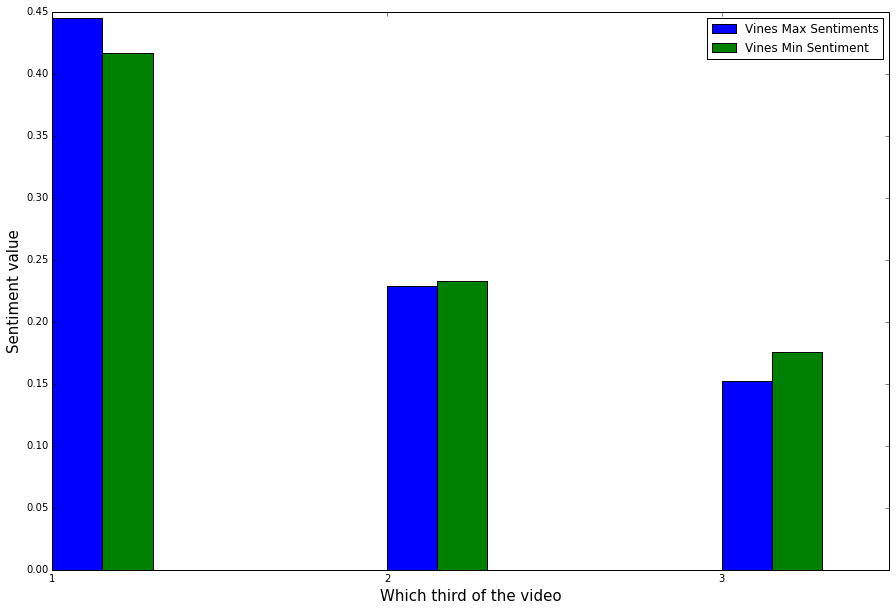
\includegraphics[width=\columnwidth]{plots/SentimentsThirds}
\caption{\textsl{ Frequency of occuranceo of maximum or minimum sentiment. For this graph, the video is considered in thirds, and the frequency of occurance of both max and min frame sentiments is plotted. }}
\label{fig:Senti_Thirds}
\end{figure} 


\begin{figure}[!htb]
\centering
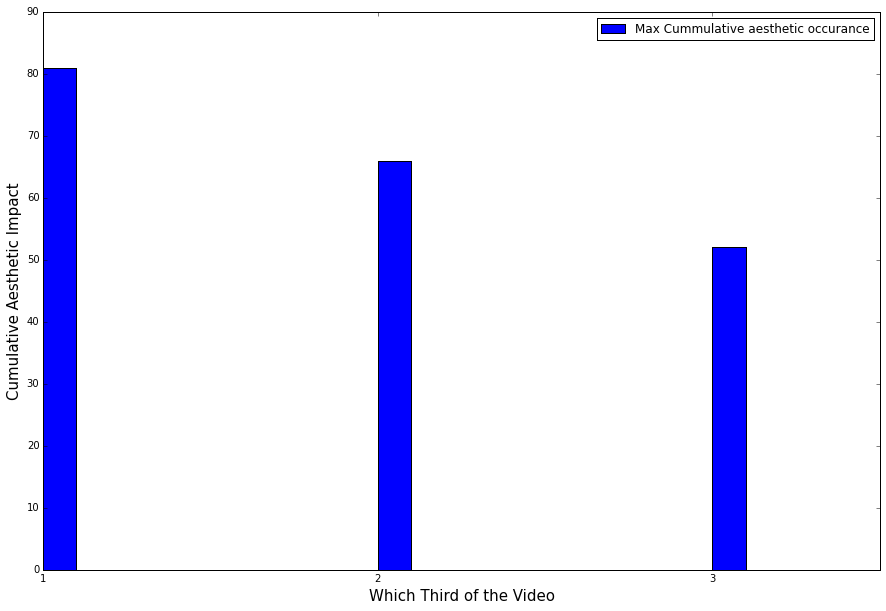
\includegraphics[width=\columnwidth]{plots/cumulativeAestheticImpact}
\caption{\textsl{ Plot of cumulative aesthetic impact of each third of the video. For this plot the videos were sampled at one frame a second, and aesthetic features were calculated at every second. Finally the features were  }}
\label{fig:Senti_Thirds}
\end{figure} 